\makeatletter
\def\input@path{{./}{../}{../../}{../../../}{../../../../}{preamble/}{../preamble/}{../../preamble/}{../../../preamble/}}
\makeatother

\input{preamble_exams.tex}
\input{graphs/uniform_linear_probability_distributions.tex}

% Keep each worked solution on one page.
\newenvironment{CThreeSolution}{%
	\par\addvspace{\medskipamount}%
	\noindent\begin{minipage}{\linewidth}%
		\setlength{\parskip}{6pt}%
}{%
	\end{minipage}\par
}

% Keep each caption and plot together. Compact axis settings apply only to solutions.
\newcommand{\CThreeSolutionGraph}[4]{%
	\par\smallskip
	\noindent\begin{minipage}{\linewidth}
		\centering\textbf{\small #1}\par
		\pgfplotsset{every axis post/.append style={
			height=3.65cm,
			xlabel={#2},ylabel={#3},
			xticklabel style={font=\small},
			yticklabel style={font=\small}
		}}
		#4
	\end{minipage}\par\smallskip
}


% A probability graph for a band split by the displayed cycle cut.
% Arguments: variable, cycle start, cycle end, pdf formula, two shaded
% domains (start:end), vertical maximum, and restart label in math mode.
% Tick choices are supplied locally.
\newcommand{\CThreeWrappedGraph}[8]{%
	\begin{center}
		\begin{tikzpicture}
			\pgfmathsetmacro{\cycleA}{#2}
			\pgfmathsetmacro{\cycleB}{#3}
			\pgfmathsetmacro{\cyclePad}{0.06*(\cycleB-\cycleA)}
			\begin{axis}[
				width=9cm,
				height=5cm,
				axis lines=left,
				xlabel={$#1$},
				ylabel={$f(#1)$},
				xmin={\cycleA-\cyclePad},
				xmax={\cycleB+\cyclePad},
				ymin=0,
				ymax=#7,
				grid=both,
				samples=241
				]
				\addplot[domain=#2:#3,draw=none,fill=blue!20,fill opacity=0.35]
				{#4}\closedcycle;
				\addplot[domain=#5,draw=none,fill=blue!65,fill opacity=0.60]
				{#4}\closedcycle;
				\addplot[domain=#6,draw=none,fill=blue!65,fill opacity=0.60]
				{#4}\closedcycle;
				\addplot[domain=#2:#3,very thick,blue] {#4};
				\coordinate (cycle left) at (rel axis cs:0.07,1);
				\coordinate (cycle right) at (rel axis cs:0.93,1);
			\end{axis}
			\draw[->,thick] ([yshift=2pt]cycle right)
				to[bend right=12] node[above,font=\small]{restart: $#8$}
				([yshift=2pt]cycle left);
		\end{tikzpicture}
	\end{center}%
}

% Rotated cycle ticks keep nearby values at the cut legible on compact graphs.
\pgfplotsset{every axis/.append style={
		scaled y ticks=false,
		xticklabel style={font=\scriptsize,rotate=35,anchor=north east}
}}

\title{Grade 11 -- Term 1 \\ C3 Practice Activity 3 with Solutions}
\author{}
\date{}

\begin{document}
	\maketitle
	\setcounter{tocdepth}{1}
	\setcounter{secnumdepth}{2}
	\phantomsection\label{toc}
	\tableofcontents
	
	\section*{Evaluated criterion}
	\begin{itemize}
		\item [\textbf{C3}] Applies circular-arc probability density functions to calculate interval probabilities using the geometry of circles and circular segments.
	\end{itemize}
	
	\section{Introduction}\label{sec:c3-introduction}
	\SectionProblemsTableOfContents{
		\SectionProblemLink{sec:c3-intro-angle-reference}{Angles on a circle: degrees and radians} \\
		\SectionProblemLink{sec:c3-intro-periodic}{Periodic variables and the cycle cut} \\
		\SectionProblemLink{sec:c3-intro-shapes}{Uniform and triangular pdf shapes} \\
		\SectionProblemLink{sec:c3-intro-method}{Nine-step geometric method}
	}\vspace{8mm}
	
	Criterion C2 constructed continuous pdfs and found probabilities from areas.
	Its uniform pdfs used rectangles, while its triangular pdfs used triangles and
	trapezoids.  Criterion C3 applies exactly those geometric methods to variables
	that repeat.  No new area method is needed; the new idea is to respect the
	cycle cut when an event passes from the end of one displayed cycle to the
	beginning of the next.
	
	The word \emph{circular} describes the \textbf{variable}: its values repeat
	after one period.  The words \emph{uniform} and \emph{triangular} describe the
	\textbf{shape of its pdf}.  A circular-uniform model therefore has a periodic
	variable and a rectangular pdf on one displayed cycle.  A
	circular-triangular model has a periodic variable and straight sides that form
	one physical triangular peak around the cycle.
	
	\subsection{Angles on a circle: degrees and radians}%
	\label{sec:c3-intro-angle-reference}
	Degrees and radians describe the same angular position using different units.
	One complete revolution is $360^\circ=2\pi$ radians, a half revolution is
	$180^\circ=\pi$, and a quarter revolution is $90^\circ=\pi/2$.  The
	conversion rules are
	\[
	\theta_{\mathrm{rad}}=\theta_{\mathrm{deg}}\frac{\pi}{180},
	\qquad
	\theta_{\mathrm{deg}}=\theta_{\mathrm{rad}}\frac{180}{\pi}.
	\]

	The standard mathematical convention measures angles counterclockwise from
	the positive horizontal axis, as shown below.  The curved arrow marks the
	positive direction of rotation.  Degree labels are on the outer ring and
	radian labels are on the inner ring so that both units remain readable.
	\begin{center}
		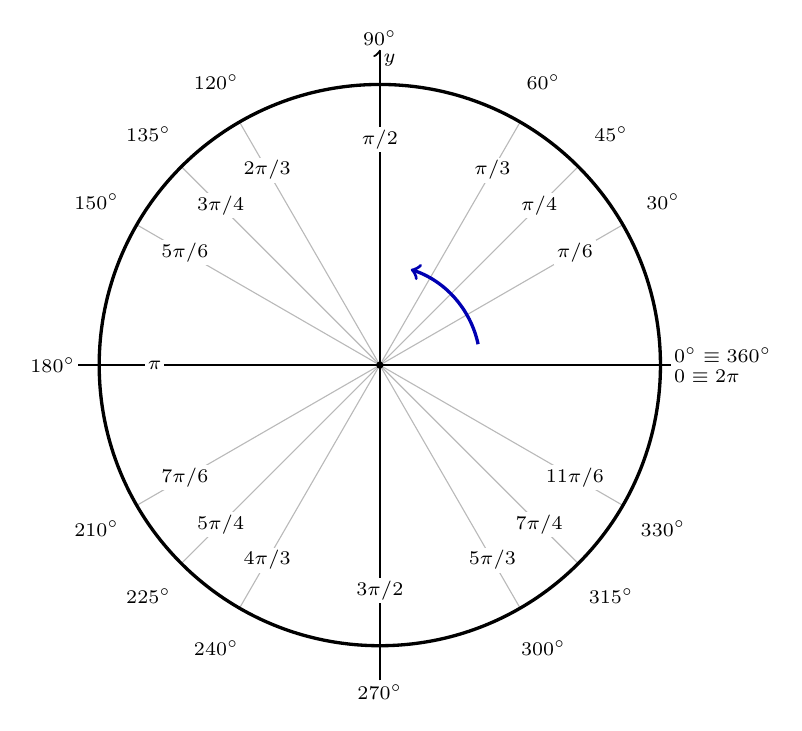
\begin{tikzpicture}[scale=0.88,
			every node/.style={font=\scriptsize,fill=white,inner sep=1pt}]
			% Standard-angle rays and the unit circle.
			\foreach \a in {0,30,45,60,90,120,135,150,180,210,225,240,270,300,315,330}
				\draw[gray!55,thin] (0,0) -- (\a:4.05);
			\draw[very thick] (0,0) circle[radius=4.05];
			\draw[->,thick] (-4.55,0) -- (4.55,0) node[below left] {$x$};
			\draw[->,thick] (0,-4.55) -- (0,4.55) node[below right] {$y$};
			\draw[->,very thick,blue!70!black]
				(12:1.45) arc[start angle=12,end angle=72,radius=1.45];


			% Outer degree ring.
			\foreach \a/\d in {
				30/30^\circ,45/45^\circ,60/60^\circ,90/90^\circ,
				120/120^\circ,135/135^\circ,150/150^\circ,180/180^\circ,
				210/210^\circ,225/225^\circ,240/240^\circ,270/270^\circ,
				300/300^\circ,315/315^\circ,330/330^\circ}
				\node at (\a:4.72) {$\d$};
			% Inner radian ring.
			\foreach \a/\r in {
				30/{\pi/6},45/{\pi/4},60/{\pi/3},90/{\pi/2},
				120/{2\pi/3},135/{3\pi/4},150/{5\pi/6},180/{\pi},
				210/{7\pi/6},225/{5\pi/4},240/{4\pi/3},270/{3\pi/2},
				300/{5\pi/3},315/{7\pi/4},330/{11\pi/6}}
				\node at (\a:3.25) {$\r$};
			% The two names for the positive horizontal ray are displayed together.
			\node[anchor=west,align=left] at (4.20,0)
				{$0^\circ\equiv360^\circ$\\[-1pt]$0\equiv2\pi$};
			\fill (0,0) circle[radius=1.5pt];
		\end{tikzpicture}
	\end{center}
	\[
	0^\circ\equiv360^\circ,
	\qquad
	0\equiv2\pi.
	\]
	Later compass contexts may measure angles clockwise from north rather than
	counterclockwise from the positive horizontal axis.  This changes the chosen
	reference direction and direction of increase, but the degree--radian
	conversions remain unchanged.

	The standard angles in the diagram are collected in this compact reference
	table.
	\begin{center}
		\small
		\renewcommand{\arraystretch}{1.15}
		\begin{tabular}{c|c@{\qquad}c|c@{\qquad}c|c}
			\textbf{Degrees} & \textbf{Radians} & \textbf{Degrees} & \textbf{Radians}
				& \textbf{Degrees} & \textbf{Radians} \\ \hline
			$0^\circ$   & $0$       & $120^\circ$ & $2\pi/3$  & $240^\circ$ & $4\pi/3$  \\
			$30^\circ$  & $\pi/6$   & $135^\circ$ & $3\pi/4$  & $270^\circ$ & $3\pi/2$  \\
			$45^\circ$  & $\pi/4$   & $150^\circ$ & $5\pi/6$  & $300^\circ$ & $5\pi/3$  \\
			$60^\circ$  & $\pi/3$   & $180^\circ$ & $\pi$     & $315^\circ$ & $7\pi/4$  \\
			$90^\circ$  & $\pi/2$   & $210^\circ$ & $7\pi/6$  & $330^\circ$ & $11\pi/6$ \\
			                 &           & $225^\circ$ & $5\pi/4$  & $360^\circ$ & $2\pi$
		\end{tabular}
	\end{center}

	For circular probability, angular widths can be measured in either degrees or
	radians, but all angles in one calculation must use consistent units.  One
	complete cycle has width $360^\circ$ or $2\pi$, and its equivalent endpoints
	represent the same physical direction.
	\secInicio[sec:c3-intro-angle-reference][sec:c3-introduction]

	\subsection{Periodic variables and the cycle cut}\label{sec:c3-intro-periodic}
	Compass direction repeats after one revolution, time of day repeats after one
	day, and rotation repeats when a device returns to its starting orientation.
	For example,
	\[
	0^\circ\equiv360^\circ,
	\qquad 0\text{ h}\equiv24\text{ h},
	\qquad f(x+P)=f(x),
	\]
	where $P$ is the period length.  For radians, $P=2\pi$; for degrees,
	$P=360^\circ$; and for time of day in hours, $P=24$ h.
	
	Displaying one circle as an interval requires a \emph{cut}.  For example,
	$[0^\circ,360^\circ)$ cuts the compass at north.  The interval has a written
	beginning and end, but the physical compass has no endpoint.  Thus
	$359^\circ$ and $1^\circ$ are only $2^\circ$ apart across the cut.  Likewise,
	23:59 and 00:01 are close times even though their recorded numbers lie on
	opposite sides of the midnight cut.
	
	The displayed interval is a recording convention, not a statement that the
	model stops beyond its endpoints.  Consequently, do not automatically add an
	``otherwise'' branch with zero density.  Write the pdf on one chosen cycle and
	state its periodic extension.  The equivalent endpoints describe the same
	physical value, and a wrapped event must be split only for area bookkeeping.
	\secInicio[sec:c3-intro-periodic][sec:c3-introduction]
	
	\subsection{Uniform and triangular pdf shapes}\label{sec:c3-intro-shapes}
	The only area formulas required in this activity are
	\[
	A_{\text{rectangle}}=bh,\qquad
	A_{\text{triangle}}=\frac12bh,\qquad
	A_{\text{trapezoid}}=\frac12(h_1+h_2)b.
	\]
	Here $b$ is horizontal width and each $h$ is a pdf height.  A probability is
	the area of its shaded region, and the area over one complete cycle is $1$.
	
	For a uniform pdf on a period of length $P$, the whole cycle is a rectangle:
	\[
	\text{Uniform: }1=Ph,\qquad h=\frac1P.
	\]
	Equal-width arcs or time bands therefore have equal probabilities.  This is a
	reasonable model when a controlled randomizer deliberately gives every part
	of a cycle the same chance, or when the model is explicitly introduced as a
	baseline for comparison.  Periodicity alone does not imply uniformity.
	
	For a triangular pdf on a period of length $P$, the complete physical peak has
	base $P$ and height $H$:
	\[
	\text{Triangular: }1=\frac12PH,\qquad H=\frac2P.
	\]
	If the mode lies inside the displayed interval, the graph rises to $H$ and
	falls to zero at the cut.  Straight-side heights can be found from line
	equations, similar triangles, or proportions, exactly as in C2.
	
	If the physical peak lies at the cut, the unwrapped graph shows two triangular
	pieces: one descends from the peak at the left endpoint, and the other rises
	to the same peak at the equivalent right endpoint.  If their bases are
	$b_1$ and $b_2$, then $b_1+b_2=P$ and
	\[
	\underbrace{\frac12b_1H}_{\text{first displayed piece}}
	+\underbrace{\frac12b_2H}_{\text{second displayed piece}}
	=\frac12PH=1.
	\]
	These are not two physical modes.  They are the two displayed parts of one
	peak joined across the cut.
	\secInicio[sec:c3-intro-shapes][sec:c3-introduction]
	
	\subsection{Nine-step geometric method}\label{sec:c3-intro-method}
	Use this routine for every problem.
	\begin{enumerate}
		\item Define the variable, units, period, and chosen cut.\par
		\item Identify the rectangular or triangular shape.\par
		\item Use total area $1$ to find unknown heights.\par
		\item Find intermediate heights with line equations, similar triangles, or
		proportions.\par
		\item Write the pdf on one cycle and state its periodic extension.\par
		\item Shade the requested region.\par
		\item Split at the cycle cut or pdf breakpoints.\par
		\item Add geometric areas, or subtract simple outside regions from $1$.\par
		\item Check $0\le P(\text{event})\le1$ and interpret the result.\par
	\end{enumerate}
	
	A circle has no intrinsic left or right tail.  The context must name the
	direction and the cut.  For example, ``the clockwise sector from $300^\circ$
	to the end of the displayed cycle'' means $[300^\circ,360^\circ)$.  A band
	within $30^\circ$ of the cut is written as the wrapped event
	\[
	[330^\circ,360^\circ)\cup[0^\circ,30^\circ].
	\]
	The two written pieces are disjoint, so their labelled geometric areas are
	added.
	\secInicio[sec:c3-intro-method][sec:c3-introduction]
	
	\newpage
	\section{Circular Uniform Distributions}\label{sec:c3-uniform}
	\SectionProblemsTableOfContents{
		\SectionProblemLink{sec:c3-uniform-sensor}{Random sensor orientation} \\
		\SectionProblemLink{sec:c3-uniform-check}{Random daily system-check time} \\
		\SectionProblemLink{sec:c3-uniform-device}{Randomized rotating-device direction}
	}
	
	\subsection{Random sensor orientation}\label{sec:c3-uniform-sensor}
	A university student in Bogot\'a is testing an augmented-reality app that places
	an object around the user.  Let $\Theta$ be the object's clockwise orientation
	from the app's reference mark, measured in radians and recorded on $[0,2\pi)$.
	Orientation is periodic because one full rotation returns to the same direction,
	so $0$ and $2\pi$ are equivalent.
	
	For each test, the app generates a direction by controlled randomization that
	gives equal chances to equal-width arcs.  A circular-uniform pdf is therefore
	reasonable by design.  The student checks the clockwise sector from $3\pi/2$
	to the cut as one interface-test sector, and the wrapped band within $\pi/6$
	of the reference mark as the app's alignment band.
	
	% The actual height is used to draw the shape but hidden from students.
	\begingroup
	\pgfplotsset{every axis/.append style={
			xticklabels={$0$,${\pi}/{6}$,${3\pi}/{2}$,${11\pi}/{6}$,$2\pi\equiv0$},
			yticklabels=\empty}}
	\CtwoProbGraph[\theta]{0}{6.283185307}{1/(2*pi)}{0}{6.283185307}
	{0,0.523598776,4.712388980,5.759586532,6.283185307}{0.20}
	\endgroup
	
	\textbf{Questions/Tasks.}
	\begin{enumerate}
		\CriterionTask{subsec:c3-uniform-sensor-a}{3.1}{Construct the complete periodic pdf of $\Theta$ from the calibration narrative, using total rectangular area $1$ to find its height and stating the period.}
		\CriterionTask{subsec:c3-uniform-sensor-b}{3.2}{Calculate the interface-test tail probability for the clockwise sector from $3\pi/2$ to the end of the displayed cycle.}
		\CriterionTask{subsec:c3-uniform-sensor-c}{3.3}{Calculate the alignment-band probability within $\pi/6$ of the reference mark, crossing the cycle cut.}
	\end{enumerate}
	
	\begin{CThreeSolution}
		\subsubsection*{C3.1 - Construct the periodic pdf.}
		\label{subsec:c3-uniform-sensor-a}
		Let $\Theta$ be the app object's clockwise orientation in radians. One full
		turn has period $2\pi$ rad. Use $[0,2\pi)$, cut at the app's reference mark
		($0\equiv2\pi$).

		Equal-width arcs are equally likely, so the density is a rectangle of
		height $h$. Its area over one cycle gives
		\[
		1=(2\pi)h \quad\Longrightarrow\quad h=\frac{1}{2\pi}\ \mathrm{rad}^{-1}.
		\]
		On the chosen cycle and under periodic extension, respectively,
		\[
		f_{\Theta}(\theta)=\frac{1}{2\pi}\quad (0\le\theta<2\pi),
		\qquad f_{\Theta}(\theta+2\pi)=f_{\Theta}(\theta).
		\]
	\end{CThreeSolution}

	\newpage
	\begin{CThreeSolution}
		\subsubsection*{C3.2 - Calculate the clockwise tail.}
		\label{subsec:c3-uniform-sensor-b}
		Moving clockwise from $3\pi/2$ to the reference mark gives
		$E=[3\pi/2,2\pi)$ on the displayed cycle.
		\CThreeSolutionGraph{Interface-test sector up to the cut ($2\pi\equiv0$)}
		{$\theta$ (rad)}{$f_{\Theta}(\theta)$}{
			\pgfplotsset{every axis/.append style={
				xticklabels={$0$,$3\pi/2$,$2\pi$},
				ytick={0,0.159154943},yticklabels={$0$,$1/(2\pi)$}}}
			\CtwoProbGraph[\theta]{0}{6.283185307}{1/(2*pi)}{4.712388980}{6.283185307}
			{0,4.712388980,6.283185307}{0.20}
		}
		The shaded rectangle has height $1/(2\pi)$ per radian, so its area is
		the favourable angular width divided by the full turn.
		\[
		P(\Theta\in E)
		=\left(2\pi-\frac{3\pi}{2}\right)\frac{1}{2\pi}
		=\frac{\pi/2}{2\pi}=\boxed{\frac14}=25\%.
		\]
		One quarter of the app's randomized orientations fall in the interface-test sector.
	\end{CThreeSolution}

	\begin{CThreeSolution}
		\subsubsection*{C3.3 - Calculate the wrapped alignment band.}
		\label{subsec:c3-uniform-sensor-c}
		The tolerance is $\pi/6$ rad ($30^\circ$) on each side of the reference
		mark. In radians, the counterclockwise side is $[11\pi/6,2\pi)$ and the
		clockwise side is $[0,\pi/6]$. Their union is the alignment band.
		\CThreeSolutionGraph{Two sides of the reference mark ($2\pi\equiv0$)}
		{$\theta$ (rad)}{$f_{\Theta}(\theta)$}{
			\pgfplotsset{every axis/.append style={
				xtick={0,0.523598776,5.759586532,6.283185307},
				xticklabels={$0$,$\pi/6$,$11\pi/6$,$2\pi$},
				ytick={0,0.159154943},yticklabels={$0$,$1/(2\pi)$}}}
			\CThreeWrappedGraph{\theta}{0}{6.283185307}{1/(2*pi)}
			{0:0.523598776}{5.759586532:6.283185307}{0.20}{2\pi\equiv 0}
		}
		Each shaded rectangle is $\pi/6$ rad wide and has height $1/(2\pi)$ per radian.
		Adding their areas gives the total favourable angular width divided by $2\pi$.
		\[
		P(\text{alignment band})
		=\frac{\pi}{6}\cdot\frac{1}{2\pi}+\frac{\pi}{6}\cdot\frac{1}{2\pi}
		=\frac{\pi/6+\pi/6}{2\pi}=\boxed{\frac16}\approx16.7\%.
		\]
		About $16.7\%$ of randomized app orientations meet the alignment tolerance.
	\end{CThreeSolution}

	\secInicio[sec:c3-uniform-sensor][sec:c3-uniform]
	
	\newpage
	\subsection{Random daily system-check time}\label{sec:c3-uniform-check}
	A student team in Bogot\'a maintains a digital platform for a university
	project and schedules one automated system check each day.  Let $T$ be the
	check's time of day in hours, recorded on $[0,24)$ with the cut at midnight.
	Time of day is periodic because the 24-hour clock returns to the same time
	after one day: $0$ h and $24$ h are equivalent.
	
	To avoid favoring any particular time window, the scheduler uses controlled
	randomization that gives equal chances to equal-length intervals.  This makes
	a circular-uniform model reasonable.  The team studies the probability that
	a check occurs from 18:00 to midnight and the probability that it occurs from
	21:00 through 03:00, when a check would fall outside typical daytime work.
	
	\begingroup
	\pgfplotsset{every axis/.append style={
			xticklabels={$0$,$3$,$18$,$21$,$24\equiv0$},yticklabels=\empty}}
	\CtwoProbGraph[t]{0}{24}{1/24}{0}{24}{0,3,18,21,24}{0.052}
	\endgroup
	
	\textbf{Questions/Tasks.}
	\begin{enumerate}
		\CriterionTask{subsec:c3-uniform-check-a}{3.1}{Construct the complete periodic pdf of $T$ from the scheduler narrative, using total rectangular area $1$ to find its height and stating the period.}
		\CriterionTask{subsec:c3-uniform-check-b}{3.2}{Calculate the evening tail probability from 18:00 to the end of the displayed day.}
		\CriterionTask{subsec:c3-uniform-check-c}{3.3}{Calculate the overnight band probability from 21:00 through 03:00, crossing midnight.}
	\end{enumerate}
	
	\begin{CThreeSolution}
		\subsubsection*{C3.1 - Construct the periodic pdf.}
		\label{subsec:c3-uniform-check-a}
		Let $T$ be the automated check's time of day in hours. The period is $24$ h.
		Use $[0,24)$, cut at midnight ($0$ h and $24$ h).

		Equal-length time windows are equally likely, so the density is a rectangle
		of height $h$. Its area over one day gives
		\[
		1=24h \quad\Longrightarrow\quad h=\frac{1}{24}\ \mathrm{h}^{-1}.
		\]
		On the chosen cycle and under periodic extension, respectively,
		\[
		f_T(t)=\frac{1}{24}\quad (0\le t<24),
		\qquad f_T(t+24)=f_T(t).
		\]
	\end{CThreeSolution}

	\newpage
	\begin{CThreeSolution}
		\subsubsection*{C3.2 - Calculate the late-cycle tail.}
		\label{subsec:c3-uniform-check-b}
		In hours on $[0,24)$, the evening tail from 18:00 to midnight is $[18,24)$.
		\CThreeSolutionGraph{Evening window up to midnight ($24\equiv0$)}
		{$t$ (h)}{$f_T(t)$}{
			\pgfplotsset{every axis/.append style={
				xticklabels={$0$,$18$,$24$},
				ytick={0,0.041666667},yticklabels={$0$,$1/24$}}}
			\CtwoProbGraph[t]{0}{24}{1/24}{18}{24}{0,18,24}{0.052}
		}
		The shaded rectangle is $6$ h wide and $1/24$ per hour high. Its area is
		the favourable time length divided by $24$ h.
		\[
		P(18\le T<24)=(24-18)\frac{1}{24}=\frac{6}{24}=\boxed{\frac14}=25\%.
		\]
		One quarter of randomized system checks are expected between 18:00 and midnight.
	\end{CThreeSolution}

	\begin{CThreeSolution}
		\subsubsection*{C3.3 - Calculate the overnight band.}
		\label{subsec:c3-uniform-check-c}
		On the hour scale, 21:00 is $t=21$ and 03:00 is $t=3$. The overnight
		window runs from 21:00 to midnight and then from midnight to 03:00,
		giving $[21,24)\cup[0,3]$.
		\CThreeSolutionGraph{Three hours on each side of midnight ($24\equiv0$)}
		{$t$ (h)}{$f_T(t)$}{
			\pgfplotsset{every axis/.append style={
				xtick={0,3,21,24},xticklabels={$0$,$3$,$21$,$24$},
				ytick={0,0.041666667},yticklabels={$0$,$1/24$}}}
			\CThreeWrappedGraph{t}{0}{24}{1/24}{0:3}{21:24}{0.052}{24\equiv 0}
		}
		The shaded rectangles have the same height, $1/24$ per hour. Their combined
		area is the total favourable time length divided by $24$ h.
		\[
		P(\text{overnight band})=(24-21)\frac{1}{24}+(3-0)\frac{1}{24}
		=\frac{3+3}{24}=\boxed{\frac14}=25\%.
		\]
		One quarter of randomized system checks are expected in the 21:00--03:00 window.
	\end{CThreeSolution}

	\secInicio[sec:c3-uniform-check][sec:c3-uniform]
	
	\newpage
	\subsection{Randomized rotating-device direction}\label{sec:c3-uniform-device}
	At a university event in Bogot\'a, a motorized camera is used to create
	$360^\circ$ video clips.  It records its direction $D$ in degrees clockwise from
	its home mark on $[0^\circ,360^\circ)$.  Direction is periodic: after a
	$360^\circ$ rotation the camera has returned to its home direction, so the
	displayed endpoints are equivalent.
	
	For each clip, the controller deliberately randomizes the starting direction
	with no preferred sector, making a circular-uniform model appropriate by
	design.  The clockwise sector from $300^\circ$ to the cut is the side where the
	camera approaches its support cable, while the $120^\circ$--$210^\circ$ sector
	frames the event backdrop.  The two probabilities help plan the camera setup.
	
	\begingroup
	\pgfplotsset{every axis/.append style={
			xticklabels={$0^\circ$,$120^\circ$,$210^\circ$,$300^\circ$,$360^\circ\equiv0^\circ$},
			yticklabels=\empty}}
	\CtwoProbGraph[d]{0}{360}{1/360}{0}{360}{0,120,210,300,360}{0.0035}
	\endgroup
	
	\textbf{Questions/Tasks.}
	\begin{enumerate}
		\CriterionTask{subsec:c3-uniform-device-a}{3.1}{Construct the complete periodic pdf of $D$ from the controller narrative, using total rectangular area $1$ to find its height and stating the period.}
		\CriterionTask{subsec:c3-uniform-device-b}{3.2}{Calculate the support-cable tail probability for the clockwise sector from $300^\circ$ to the end of the displayed cycle.}
		\CriterionTask{subsec:c3-uniform-device-c}{3.3}{Calculate the backdrop-viewing band probability for the target sector from $120^\circ$ through $210^\circ$.}
	\end{enumerate}
	
	\begin{CThreeSolution}
		\subsubsection*{C3.1 - Construct the periodic pdf.}
		\label{subsec:c3-uniform-device-a}
		Let $D$ be the camera's starting direction in degrees clockwise from its home
		mark. The period is $360^\circ$. Use $[0^\circ,360^\circ)$, cut at the home mark
		($0^\circ\equiv360^\circ$).

		The controller gives equal-width sectors equal probabilities, so the density
		is a rectangle of height $h$. Its area over one turn gives
		\[
		1=360h \quad\Longrightarrow\quad h=\frac{1}{360}\text{ per degree}.
		\]
		With $d$ measured in degrees, the density on one cycle and its periodic
		extension are
		\[
		f_D(d)=\frac{1}{360}\quad (0\le d<360),
		\qquad f_D(d+360)=f_D(d).
		\]
	\end{CThreeSolution}

	\newpage
	\begin{CThreeSolution}
		\subsubsection*{C3.2 - Calculate the directional tail.}
		\label{subsec:c3-uniform-device-b}
		The support-cable sector runs clockwise from $300^\circ$ to the home mark.
		On the chosen cycle it is $[300^\circ,360^\circ)$.
		\CThreeSolutionGraph{Support-cable sector up to the cut ($360^\circ\equiv0^\circ$)}
		{$d$ (degrees)}{$f_D(d)$}{
			\pgfplotsset{every axis/.append style={
				xticklabels={$0^\circ$,$300^\circ$,$360^\circ$},
				ytick={0,0.002777778},yticklabels={$0$,$1/360$}}}
			\CtwoProbGraph[d]{0}{360}{1/360}{300}{360}{0,300,360}{0.0035}
		}
		The shaded rectangle has height $1/360$ per degree, so its area is
		the favourable angular width divided by the full turn.
		\[
		P(300^\circ\le D<360^\circ)=(360-300)\frac{1}{360}
		=\frac{60}{360}=\boxed{\frac16}\approx16.7\%.
		\]
		About $16.7\%$ of randomized camera starts point into the support-cable sector.
	\end{CThreeSolution}

	\begin{CThreeSolution}
		\subsubsection*{C3.3 - Calculate the target sector.}
		\label{subsec:c3-uniform-device-c}
		The backdrop-viewing sector occupies the single interval $[120^\circ,210^\circ]$.
		\CThreeSolutionGraph{Backdrop-viewing sector within one cycle}
		{$d$ (degrees)}{$f_D(d)$}{
			\pgfplotsset{every axis/.append style={
				xticklabels={$0^\circ$,$120^\circ$,$210^\circ$,$360^\circ$},
				ytick={0,0.002777778},yticklabels={$0$,$1/360$}}}
			\CtwoProbGraph[d]{0}{360}{1/360}{120}{210}{0,120,210,360}{0.0035}
		}
		The shaded rectangle has height $1/360$ per degree, so its area is
		the favourable angular width divided by the full turn.
		\[
		P(120^\circ\le D\le210^\circ)=(210-120)\frac{1}{360}
		=\frac{90}{360}=\boxed{\frac14}=25\%.
		\]
		One quarter of randomized camera starts point toward the backdrop sector.
	\end{CThreeSolution}

	\secInicio[sec:c3-uniform-device][sec:c3-uniform]
	
	\newpage
	\section{Circular Triangular Distributions}\label{sec:c3-triangular}
	\SectionProblemsTableOfContents{
		\SectionProblemLink{sec:c3-triangular-scanner}{Scanner direction with an interior mode} \\
		\SectionProblemLink{sec:c3-triangular-activity}{Daily peak-activity time} \\
		\SectionProblemLink{sec:c3-triangular-north}{Direction with its peak at the cut}
	}
	
	\subsection{Scanner direction with an interior mode}\label{sec:c3-triangular-scanner}
	In a technical-education robotics lab in Bogot\'a, a motorized scanner records
	its clockwise direction $S$ in degrees on $[0^\circ,360^\circ)$, with the cut at
	north.  Direction is periodic because $0^\circ$ and $360^\circ$ are the same
	physical direction.
	
	For a practice scan, the programmed profile makes north least likely, increases
	the direction density at a constant rate to a preferred direction of
	$120^\circ$, and then decreases it at a constant rate back to zero at the cut.
	A circular-triangular pdf is reasonable because the programmed profile has one
	preferred direction and straight changes on both sides.  The sector from
	$240^\circ$ to the cut faces a reflective window, while the
	$60^\circ$--$240^\circ$ band covers the project-display area being scanned.
	
	\begingroup
	\pgfplotsset{every axis/.append style={
			xticklabels={$0^\circ$,$60^\circ$,$120^\circ$,$240^\circ$,$360^\circ\equiv0^\circ$},
			yticklabels=\empty}}
	\COneGraph[s]{0}{360}
	{(x<=120)*(x/21600)+(x>120)*((360-x)/43200)}
	{0}{360}{0,60,120,240,360}{0.0065}
	\endgroup
	
	\textbf{Questions/Tasks.}
	\begin{enumerate}
		\CriterionTask{subsec:c3-triangular-scanner-a}{3.1}{Construct the complete periodic pdf of $S$ from the scan profile, using total triangular area $1$ to find all heights and stating the period.}
		\CriterionTask{subsec:c3-triangular-scanner-b}{3.2}{Calculate the reflective-window tail probability for the clockwise sector from $240^\circ$ to the end of the displayed cycle.}
		\CriterionTask{subsec:c3-triangular-scanner-c}{3.3}{Calculate the project-display band probability from $60^\circ$ through $240^\circ$.}
	\end{enumerate}
	
	\begin{CThreeSolution}
		\subsubsection*{C3.1 - Construct the periodic pdf.}
		\label{subsec:c3-triangular-scanner-a}
		Let $S$ be the scanner's clockwise direction in degrees from north. Its period
		is $360^\circ$. Use $[0^\circ,360^\circ)$, cut at north
		($0^\circ\equiv360^\circ$).

		The density forms a triangle with zero height at the cut and a peak $H$ at
		$120^\circ$. Its area over one turn gives
		\[
		1=\frac12(360)H\quad\Longrightarrow\quad H=\frac{1}{180}\text{ per degree}.
		\]
		The rising side starts at zero and has slope $H/120=1/21600$, giving
		$s/21600$. The falling side ends at zero and has slope
		$-H/(360-120)=-1/43200$, giving $(360-s)/43200$.
		With $s$ measured in degrees, the density and its extension are
		\[
		f_S(s)=
		\begin{cases}
			\dfrac{s}{21600},&0\le s\le120,\\[2mm]
			\dfrac{360-s}{43200},&120<s<360,
		\end{cases}
		\qquad f_S(s+360)=f_S(s).
		\]
	\end{CThreeSolution}

	\newpage
	\begin{CThreeSolution}
		\subsubsection*{C3.2 - Calculate the reflective-window tail.}
		\label{subsec:c3-triangular-scanner-b}
		The reflective-window sector runs clockwise from $240^\circ$ to north,
		so it is $[240^\circ,360^\circ)$ on the chosen cycle.
		\CThreeSolutionGraph{The reflective-window tail is a triangle}
		{$s$ (degrees)}{$f_S(s)$}{
			\pgfplotsset{every axis/.append style={
				xticklabels={$0^\circ$,$120^\circ$,$240^\circ$,$360^\circ$},
				ytick={0,0.002777778,0.005555556},yticklabels={$0$,$1/360$,$1/180$}}}
			\COneGraph[s]{0}{360}{(x<=120)*(x/21600)+(x>120)*((360-x)/43200)}
			{240}{360}{0,120,240,360}{0.0065}
		}
		The falling branch gives $f_S(240)=(360-240)/43200=1/360$.
		At $360^\circ\equiv0^\circ$ the height is zero. The shaded triangle has area
		\[
		P(240^\circ\le S<360^\circ)=\frac12(360-240)\frac{1}{360}
		=\boxed{\frac16}\approx16.7\%.
		\]
		About $16.7\%$ of programmed scans point toward the reflective-window sector.
	\end{CThreeSolution}

	\begin{CThreeSolution}
		\subsubsection*{C3.3 - Calculate the project-display band.}
		\label{subsec:c3-triangular-scanner-c}
		The project-display band $[60^\circ,240^\circ]$ crosses the peak at
		$120^\circ$. Split the band there into $[60^\circ,120^\circ]$ and
		$[120^\circ,240^\circ]$.
		\CThreeSolutionGraph{Two trapezoids meet at the $120^\circ$ peak}
		{$s$ (degrees)}{$f_S(s)$}{
			\pgfplotsset{every axis/.append style={
				xticklabels={$0^\circ$,$60^\circ$,$120^\circ$,$240^\circ$,$360^\circ$},
				after end axis/.code={\draw[dashed,thick] (axis cs:120,0) -- (axis cs:120,1/180);},
				ytick={0,0.002777778,0.005555556},yticklabels={$0$,$1/360$,$1/180$}}}
			\COneGraph[s]{0}{360}{(x<=120)*(x/21600)+(x>120)*((360-x)/43200)}
			{60}{240}{0,60,120,240,360}{0.0065}
		}
		The rising and falling branches give the boundary heights.
		\[
		f_S(60)=\frac{60}{21600}=\frac1{360},\quad
		f_S(120)=\frac{120}{21600}=\frac1{180},\quad
		f_S(240)=\frac{360-240}{43200}=\frac1{360}.
		\]
		\[
		P(60^\circ\le S\le240^\circ)
		=\underbrace{\frac12\left(\frac1{360}+\frac1{180}\right)(120-60)}_{1/4}
		+\underbrace{\frac12\left(\frac1{180}+\frac1{360}\right)(240-120)}_{1/2}
		=\boxed{\frac34}=75\%.
		\]
		The scanner points toward the project-display area on three quarters of programmed scans.
	\end{CThreeSolution}

	\secInicio[sec:c3-triangular-scanner][sec:c3-triangular]
	
	\newpage
	\subsection{Daily peak-activity time}\label{sec:c3-triangular-activity}
	A university study platform records $T$, the time of day at which its daily
	student activity reaches its peak, in hours on $[0,24)$.  Time of day is
	periodic because the clock repeats every 24 hours and midnight is both $0$ h
	and $24$ h.  The model uses midnight as the cut and as the least likely
	peak-activity time.
	
	For this planning model, the density rises at a constant rate from zero at
	midnight to a mode at 08:00, then falls at a constant rate to zero at the next
	midnight.  A circular-triangular pdf represents this single daily peak and the
	specified straight changes.  The platform team studies peaks after 18:00 and
	the 04:00--16:00 band when planning when student activity is most likely to
	reach its daily maximum.
	
	\begingroup
	\pgfplotsset{every axis/.append style={
			xticklabels={$0$,$4$,$8$,$16$,$18$,$24\equiv0$},yticklabels=\empty}}
	\COneGraph[t]{0}{24}{(x<=8)*(x/96)+(x>8)*((24-x)/192)}
	{0}{24}{0,4,8,16,18,24}{0.095}
	\endgroup
	
	\textbf{Questions/Tasks.}
	\begin{enumerate}
		\CriterionTask{subsec:c3-triangular-activity-a}{3.1}{Construct the complete periodic pdf of $T$ from the activity narrative, using total triangular area $1$ to find all heights and stating the period.}
		\CriterionTask{subsec:c3-triangular-activity-b}{3.2}{Calculate the late-activity tail probability from 18:00 to the end of the displayed day.}
		\CriterionTask{subsec:c3-triangular-activity-c}{3.3}{Calculate the daytime-activity band probability from 04:00 through 16:00.}
	\end{enumerate}
	
	\begin{CThreeSolution}
		\subsubsection*{C3.1 - Construct the periodic pdf.}
		\label{subsec:c3-triangular-activity-a}
		Let $T$ be the time of the platform's daily activity peak, in hours. Its
		period is $24$ h. Use $[0,24)$, cut at midnight ($0$ h and $24$ h).

		The density is zero at midnight and has peak height $H$ at 08:00. The
		triangular area over one day gives
		\[
		1=\frac12(24)H\quad\Longrightarrow\quad H=\frac1{12}\ \mathrm{h}^{-1}.
		\]
		The rising side starts at zero and has slope $H/8=1/96$, giving $t/96$.
		The falling side ends at zero and has slope $-H/(24-8)=-1/192$, giving
		$(24-t)/192$. The density on one cycle and its extension are
		\[
		f_T(t)=
		\begin{cases}
			\dfrac{t}{96},&0\le t\le8,\\[2mm]
			\dfrac{24-t}{192},&8<t<24,
		\end{cases}
		\qquad f_T(t+24)=f_T(t).
		\]
	\end{CThreeSolution}

	\newpage
	\begin{CThreeSolution}
		\subsubsection*{C3.2 - Calculate the late-activity tail.}
		\label{subsec:c3-triangular-activity-b}
		On the hour scale, 18:00 to the midnight cut is the interval $[18,24)$.
		\CThreeSolutionGraph{The late-activity tail is a triangle}
		{$t$ (h)}{$f_T(t)$}{
			\pgfplotsset{every axis/.append style={
				xticklabels={$0$,$8$,$18$,$24$},
				ytick={0,0.03125,0.083333333},yticklabels={$0$,$1/32$,$1/12$}}}
			\COneGraph[t]{0}{24}{(x<=8)*(x/96)+(x>8)*((24-x)/192)}
			{18}{24}{0,8,18,24}{0.095}
		}
		The falling branch gives $f_T(18)=(24-18)/192=1/32$. At midnight,
		$24\equiv0$ and the height is zero. The shaded triangle has area
		\[
		P(18\le T<24)=\frac12(24-18)\frac1{32}=\boxed{\frac3{32}}=9.375\%.
		\]
		The platform model puts the daily peak between 18:00 and midnight on
		$9.375\%$ of days.
	\end{CThreeSolution}

	\begin{CThreeSolution}
		\subsubsection*{C3.3 - Calculate the daytime-activity band.}
		\label{subsec:c3-triangular-activity-c}
		The interval from 04:00 to 16:00 is $[4,16]$ in hours. The density changes
		slope at 08:00, so split the interval into $[4,8]$ and $[8,16]$.
		\CThreeSolutionGraph{Two trapezoids meet at the 08:00 peak}
		{$t$ (h)}{$f_T(t)$}{
			\pgfplotsset{every axis/.append style={
				xticklabels={$0$,$4$,$8$,$16$,$24$},
				after end axis/.code={\draw[dashed,thick] (axis cs:8,0) -- (axis cs:8,1/12);},
				ytick={0,0.041666667,0.083333333},yticklabels={$0$,$1/24$,$1/12$}}}
			\COneGraph[t]{0}{24}{(x<=8)*(x/96)+(x>8)*((24-x)/192)}
			{4}{16}{0,4,8,16,24}{0.095}
		}
		The rising and falling branches give the boundary heights.
		\[
		f_T(4)=\frac{4}{96}=\frac1{24},\quad
		f_T(8)=\frac{8}{96}=\frac1{12},\quad
		f_T(16)=\frac{24-16}{192}=\frac1{24}.
		\]
		\[
		P(4\le T\le16)
		=\underbrace{\frac12\left(\frac1{24}+\frac1{12}\right)(8-4)}_{1/4}
		+\underbrace{\frac12\left(\frac1{12}+\frac1{24}\right)(16-8)}_{1/2}
		=\boxed{\frac34}=75\%.
		\]
		The platform model puts the daily activity peak between 04:00 and 16:00
		on three quarters of days.
	\end{CThreeSolution}

	\secInicio[sec:c3-triangular-activity][sec:c3-triangular]
	
	\newpage
	\subsection{Direction with its peak at the cut}\label{sec:c3-triangular-north}
	At a live-music event, a programmable stage light records its direction $A$ in
	degrees clockwise from north on $[0^\circ,360^\circ)$.  Direction is periodic,
	so north is both $0^\circ$ and the equivalent endpoint $360^\circ$; the physical
	direction does not stop at the recording cut.
	
	The lighting program most strongly favors north, reduces the direction density
	at a constant rate to zero at south ($180^\circ$), and then increases it at the
	same constant rate back toward north.  A circular-triangular pdf is reasonable
	for this symmetric programmed preference.  The sector from $300^\circ$ to the
	cut covers one side of the audience area, while the band within $30^\circ$ of
	north is a narrow stage-target zone.
	
	\begingroup
	\pgfplotsset{every axis/.append style={
			xticklabels={$0^\circ$,$30^\circ$,$180^\circ$,$300^\circ$,$330^\circ$,
				$360^\circ\equiv0^\circ$},yticklabels=\empty}}
	\COneGraph[a]{0}{360}
	{(x<=180)*((180-x)/32400)+(x>180)*((x-180)/32400)}
	{0}{360}{0,30,180,300,330,360}{0.0065}
	\endgroup
	
	\textbf{Questions/Tasks.}
	\begin{enumerate}
		\CriterionTask{subsec:c3-triangular-north-a}{3.1}{Construct the complete periodic pdf of $A$, showing how two displayed triangular pieces form one physical peak at the cut, using their combined area $1$ to find all heights, and stating the period.}
		\CriterionTask{subsec:c3-triangular-north-b}{3.2}{Calculate the audience-side tail probability for the clockwise upper-end sector from $300^\circ$ to the end of the displayed cycle.}
		\CriterionTask{subsec:c3-triangular-north-c}{3.3}{Calculate the stage light's wrapped target-band probability on $[330^\circ,360^\circ)\cup[0^\circ,30^\circ]$.}
	\end{enumerate}
	
	\begin{CThreeSolution}
		\subsubsection*{C3.1 - Construct the periodic pdf.}
		\label{subsec:c3-triangular-north-a}
		Let $A$ be the stage-light direction in degrees clockwise from north.
		Its period is $360^\circ$. Use $[0^\circ,360^\circ)$, cut at north
		($0^\circ\equiv360^\circ$).

		The cut splits the physical peak $H$ between the two displayed ends. Each
		triangle has base $180^\circ$ and meets the other at zero density at south.
		The total area over one turn gives
		\[
		1=\frac12(180)H+\frac12(180)H=180H
		\quad\Longrightarrow\quad H=\frac1{180}\text{ per degree}.
		\]
		Both line segments meet at $(180,0)$. The descending slope is
		$-H/180=-1/32400$, giving $(180-a)/32400$. The ascending slope is
		$H/180=1/32400$, giving $(a-180)/32400$.
		With $a$ measured in degrees, the density and its extension are
		\[
		f_A(a)=
		\begin{cases}
			\dfrac{180-a}{32400},&0\le a\le180,\\[2mm]
			\dfrac{a-180}{32400},&180<a<360,
		\end{cases}
		\qquad f_A(a+360)=f_A(a).
		\]
	\end{CThreeSolution}

	\newpage
	\begin{CThreeSolution}
		\subsubsection*{C3.2 - Calculate the upper-end directional tail.}
		\label{subsec:c3-triangular-north-b}
		The audience-side sector runs clockwise from $300^\circ$ to the north cut.
		On the chosen cycle it is $[300^\circ,360^\circ)$.
		\CThreeSolutionGraph{The audience-side trapezoid ends at north ($360^\circ\equiv0^\circ$)}
		{$a$ (degrees)}{$f_A(a)$}{
			\pgfplotsset{every axis/.append style={
				xticklabels={$0^\circ$,$180^\circ$,$300^\circ$,$360^\circ$},
				ytick={0,0.003703704,0.005555556},yticklabels={$0$,$1/270$,$1/180$}}}
			\COneGraph[a]{0}{360}{(x<=180)*((180-x)/32400)+(x>180)*((x-180)/32400)}
			{300}{360}{0,180,300,360}{0.0065}
		}
		On the rising side, $f_A(300)=(300-180)/32400=1/270$ and the height
		approaches $(360-180)/32400=1/180$ at north. The shaded trapezoid has area
		\[
		P(300^\circ\le A<360^\circ)
		=\frac12\left(\frac1{270}+\frac1{180}\right)(360-300)
		=\boxed{\frac5{18}}\approx27.8\%.
		\]
		About $27.8\%$ of programmed stage-light directions fall in the audience-side sector.
	\end{CThreeSolution}

	\begin{CThreeSolution}
		\subsubsection*{C3.3 - Calculate the wrapped target band.}
		\label{subsec:c3-triangular-north-c}
		The target extends $30^\circ$ ($\pi/6$ rad) to each side of north.
		In degrees, the counterclockwise side is $[330^\circ,360^\circ)$ and
		the clockwise side is $[0^\circ,30^\circ]$. Their union is the target band.
		\CThreeSolutionGraph{One trapezoid on each side of north ($360^\circ\equiv0^\circ$)}
		{$a$ (degrees)}{$f_A(a)$}{
			\pgfplotsset{every axis/.append style={
				xtick={0,30,180,330,360},
				xticklabels={$0^\circ$,$30^\circ$,$180^\circ$,$330^\circ$,$360^\circ$},
				ytick={0,0.004629630,0.005555556},yticklabels={$0$,$1/216$,$1/180$}}}
			\CThreeWrappedGraph{a}{0}{360}
			{(x<=180)*((180-x)/32400)+(x>180)*((x-180)/32400)}
			{0:30}{330:360}{0.0065}{360^\circ\equiv 0^\circ}
		}
		At north, $f_A(0)=f_A(360^-)=1/180$. The other boundary heights are
		\[
		f_A(330)=\frac{330-180}{32400}=\frac1{216},
		\qquad f_A(30)=\frac{180-30}{32400}=\frac1{216}.
		\]
		Add the areas of the two $30^\circ$-wide trapezoids.
		\[
		P(\text{target band})
		=\underbrace{\frac12\left(\frac1{216}+\frac1{180}\right)(30)}_{11/72}
		+\underbrace{\frac12\left(\frac1{180}+\frac1{216}\right)(30)}_{11/72}
		=\boxed{\frac{11}{36}}\approx30.6\%.
		\]
		About $30.6\%$ of programmed stage-light directions are within $30^\circ$ of north.
	\end{CThreeSolution}

	\secInicio[sec:c3-triangular-north][sec:c3-triangular]
	
\end{document}
